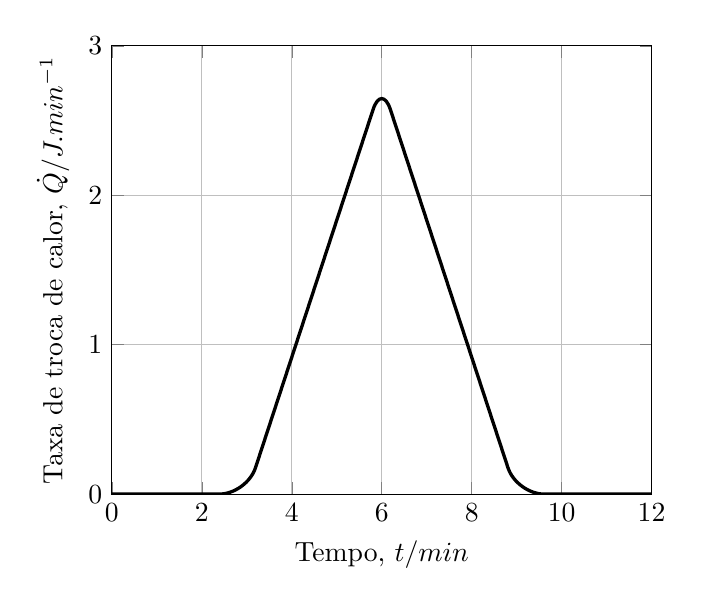
\begin{tikzpicture}
    \begin{axis}
        [
            grid = major,
            xlabel = {Tempo, $t/\si{min}$},
            ylabel = {Taxa de troca de calor, $\dot{Q}/\si{J.min^{-1}}$},
            xmin=0, xmax=12,
            ymin=0, ymax=3,
        ]
    \draw [very thick, rounded corners=1em]
        (axis cs: 0,0) --
        (axis cs: 3,0) --
        (axis cs: 6,2.75) --
        (axis cs: 9,0) --
        (axis cs: 12,0);
    \end{axis}
\end{tikzpicture}